\documentclass[a4paper,10pt, sans]{article}
\usepackage[utf8x]{inputenc}
\usepackage[spanish]{babel}
\usepackage{hyperref}
\usepackage{verbatim}
\usepackage{graphicx}
\usepackage{float}
\usepackage{wrapfig}
\usepackage{LTXtable}
%\usepackage{amsmath,amssymb,amsfonts,latexsym,cancel}
\usepackage{multicol}      %para usar varias columnas
  %uso:
  %\begin{multicols}{2}
    %texto
  %\end{multicols}
\usepackage{marvosym}

\setlength{\columnsep}{4mm}    %separación de columnas
%\usepackage{pslatex}
%\hoffset -0.75in        %cambio el margen horizontal izquierdo
%\voffset -0.9in          %cambio el margen vertical superior
\textwidth 17cm        %ancho de texto. defaut: 14cm
\textheight 25cm        %alto de texto. default: 19cm
\topmargin -1cm        %agranda el margen superior. default: 3cm
\oddsidemargin -1cm        %agranda el margen izquierdo. default: 2.5cm (4.5 si no aparece esta instrucción)
\pagestyle{empty} %{myheadins}  %numeración de pág: sin / arriba
\parskip 2mm          %X mm entre párrafos
%\parindent 0mm          %elimina sangría

\begin{document}
  

  \begin{wrapfigure}{r}{4cm}
    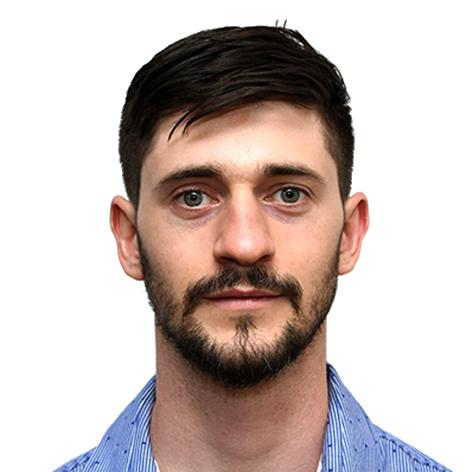
\includegraphics[height=4cm]{seba_4x4.jpg}
  \end{wrapfigure}

  \sffamily
  
  \begin{Huge}
    Sebastián Rossi
  \end{Huge}
  \\ \\
  \hspace*{0.5cm} \textit{CURRICULUM VITAE} \\
  \hspace*{0.5cm} {\textit{Actualizado: 30/01/2022}}
  
  \begin{tabular}{rl}
    \vspace{0.5cm} \\
    \large\Mobilefone & \textbf{+549 3402 507471} \\
    \large\Letter & \textbf{srossi@inti.gob.ar}
  \end{tabular}

  \vspace{0.5cm}
  \large
  \begin{table}[h!]
  \begin{tabularx}{\textwidth}{r X}
    %%%%%%%%%%%%%%%%%%%%%%%%%%%%%%%%%%%%%%%%%%%%%%%%%%%%%%%%%%%%%%%%%%%%%%%%%%%%
    \textbf{Datos Personales} & {} \\ [1ex]
      {} & Fecha de Nacimiento: 15-11-1988 \\ [1ex]
      {} & Nacionalidad: Argentino - Italiano \\ [1ex]
      {} & Domicilio: Maipú 782, (2107) Álvarez, Santa Fe, Argentina \\ \\ \hline \\

    %%%%%%%%%%%%%%%%%%%%%%%%%%%%%%%%%%%%%%%%%%%%%%%%%%%%%%%%%%%%%%%%%%%%%%%%%%%%
    
    \textbf{Educación} & {} \\ [1ex]
       (2020 - ) & \textbf{Doctorado en Ingeniería}, FCEIA, Universidad Nacional de Rosario. Tesis: Sensado y control de sistemas de siembra neumáticos. Directores: Ignacio Rubio Scola, Gastón Bourges.\\ [1ex]
       (2008 - 2014) & \textbf{Ingeniero Electrónico}. FCEIA, Universidad Nacional de Rosario.\\ \\ \hline \\
    %%%%%%%%%%%%%%%%%%%%%%%%%%%%%%%%%%%%%%%%%%%%%%%%%%%%%%%%%%%%%%%%%%%%%%%%%%%%
    \textbf{Antecedentes Laborales} & {}\\ [1ex]
      (2013 - ) & Instituto Nacional de Tecnología Industrial. Departamento de Ingeniería de Productos Industriales - Rosario.\\ \\
            
        {} & \hspace{2cm} \textit{Desarrollo de nuevas capacidades.} \\ [1ex]
        
        (2013) & Medición de distribución de temperatura y tiempos de estabilización térmica en laboratorio de calibración de bloques patrón. \\ [1ex]
        (2013 - 2014) & Desarrollo de software para la adquisición de datos por puerto serie de comparadora de bloques patrón. \\ [1ex]
        (2014 - 2015) & Desarrollo e implementación de sistema de grabación multicanal comandado por wi-fi con placas Raspberry-Pi. Aplicación: detección de impacto de semillas. \\ [1ex]
        (2015) & Desarrollo de scripts en Scilab para determinar el tiempo de impacto de diferentes tipos de semillas a partir de señales de sensores piezoeléctricos y evaluación de sistemas de siembra según norma ISO 7256. \\ [1ex]
        (2016) & Desarrollo de plataforma basada en Cortex M4 para multiples canales sincronizados de sensado para detección de impacto de semillas. \\ [1ex]
        (2016 - 2017) & Redacción de documentación para integrar el servicio de medición de deformaciones con galgas extensiométricas al sistema de gestión de calidad. \\ [1ex]
        (2017 - 2019) & Experimentación en banco de pruebas air-drill con diferentes niveles de caudal de aire, flujo de semillas, configuración de cabezal distribuidor y longitudes de mangueras de salida con semillas de soja. \\ [1ex]
        (2018) & Desarrollo de plataforma modular basada en Cortex M0 con comunicación inalámbrica para adquisición de datos multicanal para sensores piezoeléctricos y transmisores de presión. \\ [1ex]
        (2019 - 2020) & Desarrollo de software de procesamiento de imágenes en python usando la biblioteca OpenCV para detección de trayectorias de semillas en videos de alta velocidad para evaluacion de dosificadores de siembra de precisión y tubos de descarga de semillas en banco de pruebas sobre mesa vibradora. Scripts R para el análisis de los resultados. \\ [1ex]
        (2020 - 2022) & Experimentos en banco de pruebas estático para evaluación de incertidumbre en sistemas de detección de semillas y trayectorias mediante placa de impacto, sensores infrarojos y procesamiento de imágenes. \\ \\
  \end{tabularx}
  \end{table}
  
  \begin{table}[H]
  \centering
  \begin{tabularx}{\textwidth}{r X}  
        {} & \hspace{2cm} \textit{Trabajos realizados para usuarios.} \\ [1ex]
        (2015 - 2016) & Evaluación de una sembradora a chorrillo usando detección de semillas con sensores piezoeléctricos tanto en banco de pruebas como sembrando en campo, basado en ISO 7256 Parte 2. Empresa: Indecar. \\  [1ex]

        (2015 - ) & Evaluación de dosificadores de siembra de precisión y tubos de descarga de semillas con procesamiento de imágenes y sensor piezoeléctrico basado en ISO 7256 Parte 1, en banco de ensayos estático y dinámico. Empresas: Siembra Neumática, Pla, Agrometal. \\ [1ex]
        (2016 - ) & Pegado de galgas extensiométricas y medición de deformaciones en estructuras de acero. Empresas: Sola y Brusa, Ejército Argentino, Ombú, Pla, Superwalter, Acerías 4C, Randon, Hermann, Crucianelli, Agrometal, Palfinger. \\ \\ \hline \\

    \textbf{Conference papers} & {}\\ [1ex]
      {} & Gastón Bourges, Sebastian Rossi, Jorge Eliach, Mabel Azucena Medina. \textit{Evaluación experimental de un dosificador de semillas de precisión.} V CAIM 2016. Santiago del Estero, Argentina. UNSE- FCEyT- ISBN: 978-987-1676-63-7. pp: 881-891. \\  [1ex]
      {} & \textit{Tests on a precision seed meter.} (in Spanish) X Jornadas de Ciencia y Tecnología. Sede de Gobierno. UNR. Rosario, Santa Fe. \\  [1ex]
      {} & Sebastián Rossi, Ignacio Rubio Scola,Jorge J. Eliach, Gastón Bourges. \textit{Evaluación de desempeño de dosificador monograno mediante filmación y procesamiento de imágenes.} VII CAIM 2020. San Nicolás, Argentina. ISBN 978-950-42-0210-3. \\  [1ex]
      {} & Gastón Bourges, Sebastián Rossi, Ignacio Rubio, Davut Karayel. \textit{Evaluación de la incidencia de diferentes factores en la distribución de semillas de soja en sistema de transporte por aire.} VII CAIM 2020. San Nicolás, Argentina. ISBN 978-950-42-0210-3. \\ [1ex]
      {} & Ignacio Rubio Scola, Sebastián Rossi, Gastón Bourges. \textit{Air drill Seeder Distributor Head Evaluation: A Comparison between Laboratory Tests and Computational Fluid Dynamics Simulations.} Capítulo de libro: Information and Communication Technologies for Agriculture—Theme II: Data. https://doi.org/10.1007/978-3-030-84148-5_8. \\ \\ \hline \\
      
    \textbf{Idiomas} & {} \\ [1ex]
    {} & Español, lengua madre. \\ [1ex]
    {} & Inglés, Nivel intermedio. \\ \\ \hline \\
      
    \textbf{Licencia de conducir} & {} \\ [1ex]
    {} & Clases A3 y B2.\\
    
\vspace{5cm}
    
    
    
    
        
  \end{tabularx}
  \end{table}
  
\end{document}
